\subsection{Finite Difference Method}
\subsubsection{Come up with a simple one dimensional differential equation \\$\mathbf{f'(x)=g(x)\ \mathrm{on}\ \Omega=[0,1]}$ by specifying g(x) and setting appropriate boundary condition (e. g. $\mathbf{f(0) = 0}$).}
Initial assumption:
\begin{equation}
    g(x) = \cos^2(\pi x)
\end{equation}
Dirichlet boundary condition:
\begin{align}
    f(0) &= 0 \label{eq:bcs}
\end{align}

\subsubsection{Solve the obtained boundary value problem analytically. Show your solution as well
as its plot.}
\begin{align}
   \int{f'(x)\ dx} &= \int{\cos^2(\pi x)\ dx}\\
  f(x) &= \frac{x}{2}+\frac{\sin\left(2\,\pi \,x\right)}{4\,\pi } + c_1\\
  f(0) &= \frac{0}{2}+\frac{\sin\left(2\,\pi \,0\right)}{4\,\pi } + c_1 \overset{!}{=} 0\\
  \Rightarrow c_1 &= 0
\end{align}
\clearpage
The corresponding MATLAB code was imeplemented as follwing:
\begin{lstlisting}
x_cont = linspace(0,1,1000);
x_interval = [0,1];
%% Plot ODE f'(x) = cos(pi x)^2 and its solution
syms f(x)
ODE = diff(f,x) == (cos(pi.*x)).^2;
bc = f(0) == 0;
sol = dsolve(ODE,bc);

figure;
yyaxis right
plot(x_cont,(cos(pi.*x_cont)).^2,'DisplayName',['ODE (f''(x) ='...
    'cos(x \pi)^2)']); hold on
xlabel('x');
ylabel('f''(x)');
yyaxis left
fplot(sol,x_interval,'DisplayName',['Analytical Solution '...
    '(f(0)=0, ' newline 'f(x)=^{x}/_{2}+sin(2\pix)/4\pi )']);
legend;
xlabel('x');
ylabel('f(x)');
\end{lstlisting}
\begin{figure}[htb!]
    \centering
    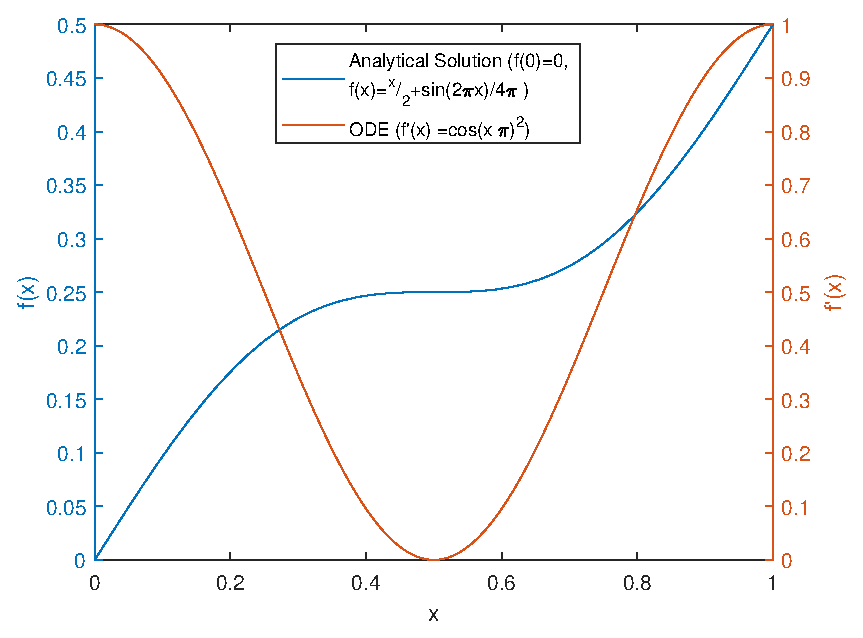
\includegraphics[width=.7\linewidth]{./homework2/img/1.eps}
    \caption{Original ODE with analytical solution}
    \label{fig:ana_sol}
\end{figure}
\subsubsection{Solve the boundary value problem using the Finite Difference Method for step h =
0.2, 0.1 and 0.01. Pick the discretization scheme yourself (forward/backward/central
difference), discretize the equation and put it into matrix form. Use linsolve() to solve
the resulting system of linear equations. Hint: unless you know what you are doing,
avoid central difference scheme.}
Choosing the \textit{forward Method} for the Finite Differences Method, where $x_i = i\ \cdot\ h\ \mathrm{with}\ i = 1,2,..., N+1\ \mathrm{and}\ N + 1= \frac{1}{h}$. 
For given h values of 0.2, 0.1 and 0.01 the dimension $M$ is 5, 10 and 100.
\begin{align}
    f'(x) &= \lim\limits_{h \rightarrow 0}{\frac{f(x+h)-f(x)}{h}}\\
    \frac{f(x+h)-f(x)}{h} &= \cos^2(\pi x) \\
    \mathrm{Discretizing:}\ \frac{f(x_{i+1})-f(x_i)}{h} &= \cos^2(\pi x_i)\\
    \mathrm{Rewriting:}\ f(x_{i+1})-f(x_i) &= h\cos^2(\pi x_i)\\
    \mathrm{Using\ Eq.}\ \ref{eq:bcs}:\ f_{1} &= f(0) = 0\\
    \underbrace{\begin{bmatrix}
    1 &   &   &   &   &   &   &   &  0\\
    -1 &  1 &   &   &   &   &   &  & \\
       &    &   &   &   &   &   &   &  \\
       &    &   &   &   &   &   &   &  \\
       &    &   &   &\ddots &\ddots &   &   &  \\
       &    &   &   &   &   &   &   &  \\
       &    &   &   &   &   &   &   &  \\
       &    &   &   &   &   &-1 &  1& \\
     0 &    &   &   &   &   &   &-1 &1\\
    \end{bmatrix}}_{M\times M}
    \underbrace{\begin{bmatrix}
f_2 \\f_3 \\ \\ \\ \vdots\\ \\ \\f_{N-1}\\ f_{N}
\end{bmatrix}}_{M\times 1}&= h \underbrace{\begin{bmatrix}
\cos^2(\pi x_1)\\\cos^2(\pi x_2)\\ \\ \\ \vdots \\ \\ \\\cos^2(\pi x_{N-2})\\\cos^2(\pi x_{N-1})
\end{bmatrix}}_{M\times 1}
\end{align}
\clearpage
The Finite Differences were computed by the following MATLAB script:
\begin{lstlisting}
%% Finite Difference Method
% Initialize Matrices
h = [0.2 0.1 0.01];
mat_size = 1./h;
A = cell(length(mat_size),1);
b = cell(length(mat_size),1);
f = cell(length(mat_size),1);
x = cell(length(mat_size),1);
fin_diff = cell(length(mat_size),1);

figure;
fplot(sol,x_interval,'DisplayName','Analytical Solution');hold on
% Populate A and b
for i = 1:length(mat_size)
    x{i} = linspace(0,1,mat_size(i))';
    A{i} = eye(mat_size(i));
    for j = 2:(mat_size(i))
        A{i}(j,j-1) = -1;
    end
    
    b{i} = double(h(i) .* ones(mat_size(i),1) .* (cos(pi .* x{i})).^2);
    
    % Evaluate Af = b
    f{i} = linsolve(double(A{i}),b{i});
    
    % Plot solution
    plot(x{i},[0;f{i}(1:end-1)],'DisplayName',['Finite Difference h = ' num2str(h(i))]);
end
legend({},'Location','northwest');
xlabel('x_i');
ylabel('f(x_i)');
\end{lstlisting}
\clearpage
\subsubsection{Plot the resulting solutions along with the exact solution you have computed in step 2}
\begin{figure}[htb!]
    \centering
    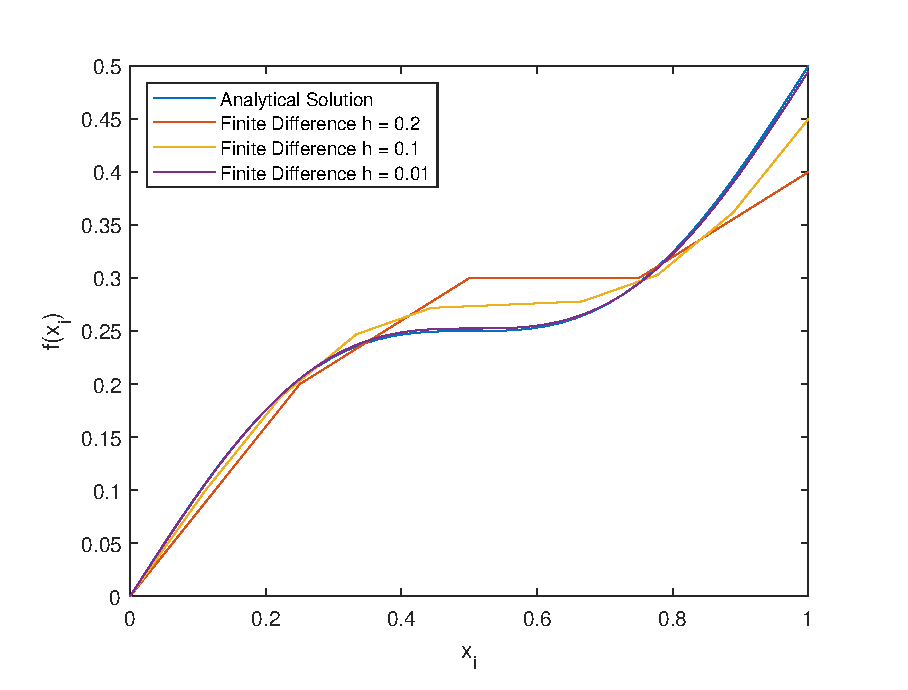
\includegraphics[width=.7\linewidth]{./homework2/img/final_FDM.eps}
    \caption{Analytical and Finite Difference solutions of the ODE}
    \label{fig:fin_diff}
\end{figure}